\section{Experimental Setup}

For the analysis of a SAC network was used the programming language Python \cite{ascher1999learning}. 
The Python language has as priority the legibility of the code under speed. 
The vast libraries and frameworks provided by Python makes it an exquisite tool for machine learning and data analysis purposes.

\subsection{ROS}

The robot operations system (ROS) is a flexible framework to write software for robots.
ROS \cite{pyo2015ros} is a collection of tools, and libraries.
ROS provides operational system standard services, like hardware's abstraction, device low level control, messages between processes and package management. 
The set of ROS processes in execution are represented by graphs architecture where the processing is performed on nodes that receive and send messages as sensors, control, state, planning, actuator and others.

Despite the importance of low latency on the robots control, ROS is not a real-time operational system, although it is possible to integrate ROS with real-time code. This lack of real-time system is being addressed on the development of ROS 2.0.

\subsection{Gazebo}

Robot simulation is an essential tool on all roboticist's toolbox.
A good simulator makes possible to test algorithms quickly, to design robots, and to train systems with artificial intelligence using realistic scenarios.
With Gazebo \cite{fairchild2016ros} is possible to simulate this environments easily and with the advantage of having an active community.
This makes Gazebo a great tool on the area of robotic simulation.

\subsection{Turtlebot}

Turtlebot is a ROS standard platform robot, and there are 3 version of the series. Turtlebots are affordable and programmable mobile robots for use in education, research, hobby, and product prototyping.
The third version was used on this project and it is shown in Fig. \ref{fig:turtlebot3}.

\begin{figure}[htbp]
\centerline{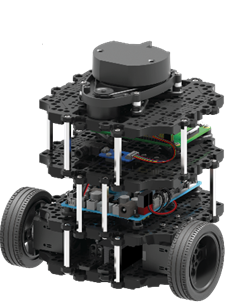
\includegraphics[width=4cm]{images/burger_real.png}}
\caption{Real Turtlebot3 version Burger.}
\label{fig:turtlebot3}
\end{figure}

The Turtlebot3 Burger uses 2 DYNAMIXEL motors series XL, for the object detection the Turtlebot3 utilize a 360 degree sensor laser LiDAR, and it has an IMU sensor for the odometry calculations.
All the control is made by the open source controller board OpenCR1.0 and Raspberry Pi 3 microprocessor.
% The Table \ref{tab1} shows all hardware specification of the Turtlebot3 version Burger.


% \begin{table}[htbp]
% \caption{Hardware Specification of the Turtlebot3 Burger}
% \begin{center}
% \begin{tabular}{|l|l|}
% \hline
% \textbf{Items}&\textbf{Specification} \\
% \hline
% Maximum translational velocity & 0.22 m/s \\
% \hline
% Maximum rotational velocity    & 2.84 rad/s (162.72 deg/s) \\
% \hline
% Maximum payload                & 15kg \\ 
% \hline
% Size (L x W x H)               & 138mm x 178mm x 192mm \\
% \hline
% Weight                         & 1kg \\
% \hline
% Threshold of climbing          & 10 mm or lower \\
% \hline
% Expected operating time        & 2h 30m \\
% \hline
% Expected charging time         & 2h 30m \\
% \hline
% SBC (Single Board Computers)   & Raspberry Pi 3 Model B and B+ \\
% \hline
% Actuator                       & DYNAMIXEL XL430-W250 \\
% \hline
% LDS(Laser Distance Sensor)     & 360 Laser Distance Sensor LDS-01 \\
% \hline
% IMU                            & \begin{tabular}[c]{@{}c@{}}Gyroscope 3 Axis\\ Accelerometer 3 Axis\\ Magnetometer 3 Axis\end{tabular} \\
% \hline
% Battery                        & \begin{tabular}[c]{@{}c@{}}Lithium polymer \\ 11.1V 1800mAh / 19.98Wh 5C \\ \end{tabular} \\
% \hline

% \end{tabular}
% \label{tab1}
% \end{center}
% \end{table}

% \subsection{OpenCV}

% Open Source Computer Vision (OpenCV) is an open source computer vision and machine learning software library.
% It is mainly used for developing advanced image processing and computer vision applications \cite{bradski2008learning}, \cite{wang2010camera}.
% OpenCV can take frames out of a video and run algorithms to get necessary information.
% It can also identify an object, recognize a face or track the movement of an object.
% It is commonly used in robotics \cite{oyama2009come}.

\subsection{Simulation Environments}

There were used two environments for the simulations. The first environment is  shown in Fig. \ref{subfig:env1}, the environment represents a free area for the robot to move.
The walls of this environment are the only things where the robot can collide.
If the mobile robot collide with the wall or any obstacle, a negative reward is given for this action and the current episode stops.
The second environment is shown in Fig. \ref{subfig:env2} and has 4 fixed obstacles.
It means that this environment is more complex in a way that the intelligent agent have to make a better strategy to not collide.
% The third environment, shown in {\color{blue}Figure} \ref{fig:environments}{\color{blue}(c)}, is more complex than the previous environments.  
% The number of walls and the mobile obstacles, represented by the white blocks, makes the environment more dynamical, approaching it to a real-world scenarios.



\begin{figure}[htbp]
    \centering
    \begin{subfigure}[b]{0.2\textwidth}
        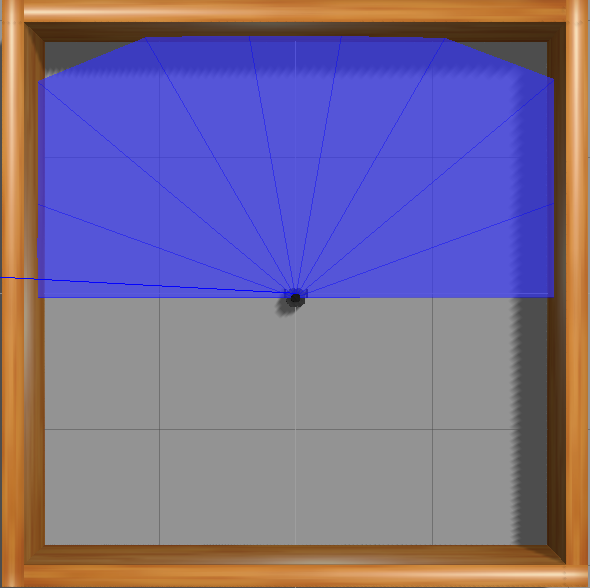
\includegraphics[width=\textwidth]{images/amb1.png}
        \caption{First environment.}
        \label{subfig:env1}
    \end{subfigure}
    ~ %add desired spacing between images, e. g. ~, \quad, \qquad, \hfill etc. 
      %(or a blank line to force the subfigure onto a new line)
    \begin{subfigure}[b]{0.2\textwidth}
        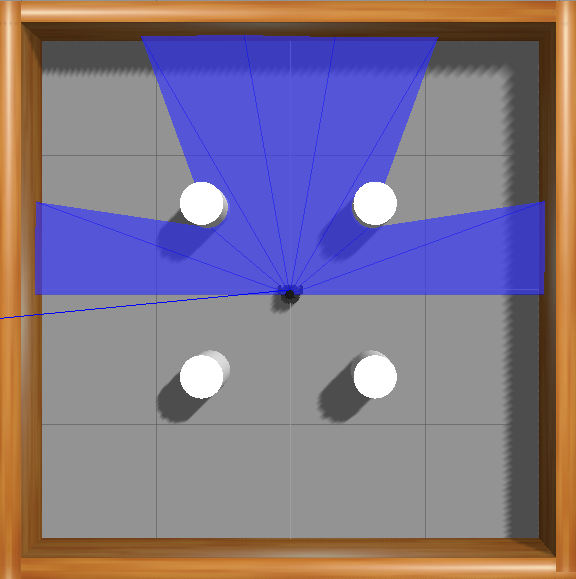
\includegraphics[width=\textwidth]{images/amb2.png}
        \caption{Second environment.}
        \label{subfig:env2}
    \end{subfigure}
    \caption{Training environments used on Gazebo simulation.}\label{fig:environments}
\end{figure}

% \begin{figure}[H]
% \centerline{\includegraphics[width=\columnwidth]{images/environments1.png}}
% \caption{Training environments used on Gazebo simulation. First environment (a), second environment (b) and third environment (c).}
% \label{fig:environments}
% \end{figure}

\subsection{Real Environments}

After training the SAC network through simulation, it will be tested in a real scenario.
The Turtlebot3, version Burger, will be used to perform this test.
Some of the necessary inputs of the network in the real environment were obtained by image processing.
The first real environment is shown in Fig. \ref{subfig:real_env1} and resembles the first simulation with no obstacles. The second environment is shown in Fig. \ref{subfig:real_env2} and it presents a complex environment similar to the second used on simulation.

\begin{figure}[htbp]
    \centering
    \begin{subfigure}[t]{0.22\textwidth}
        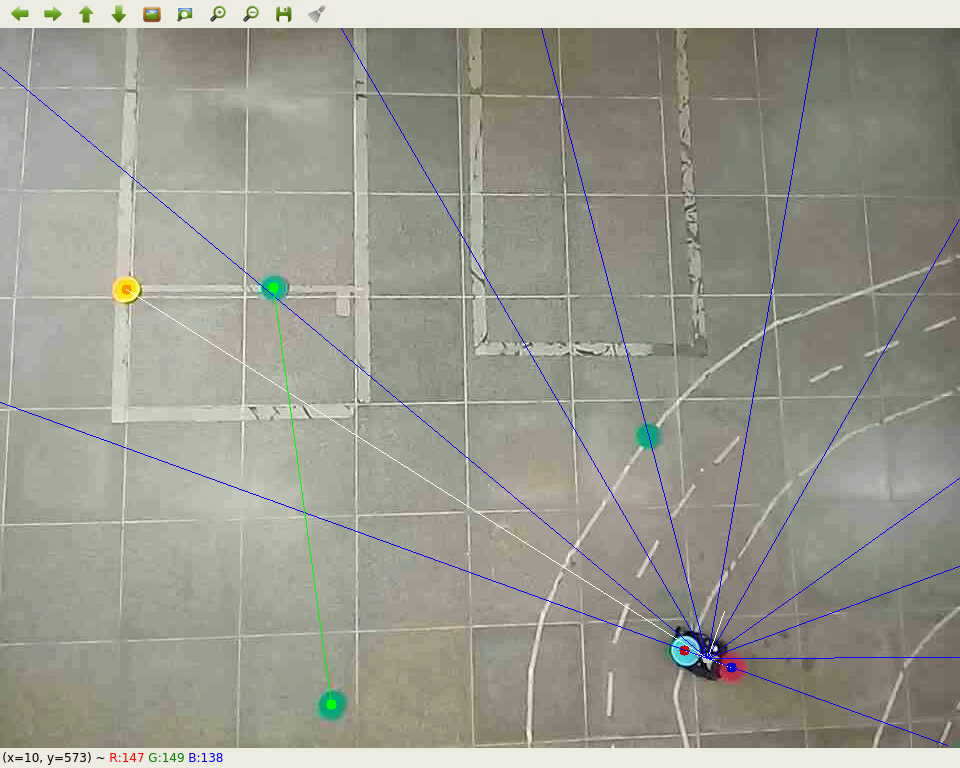
\includegraphics[width=\textwidth]{images/test_env1/1.png}
        \caption{First real environment.}
        \label{subfig:real_env1}
    \end{subfigure}
    ~
    \begin{subfigure}[t]{0.22\textwidth}
        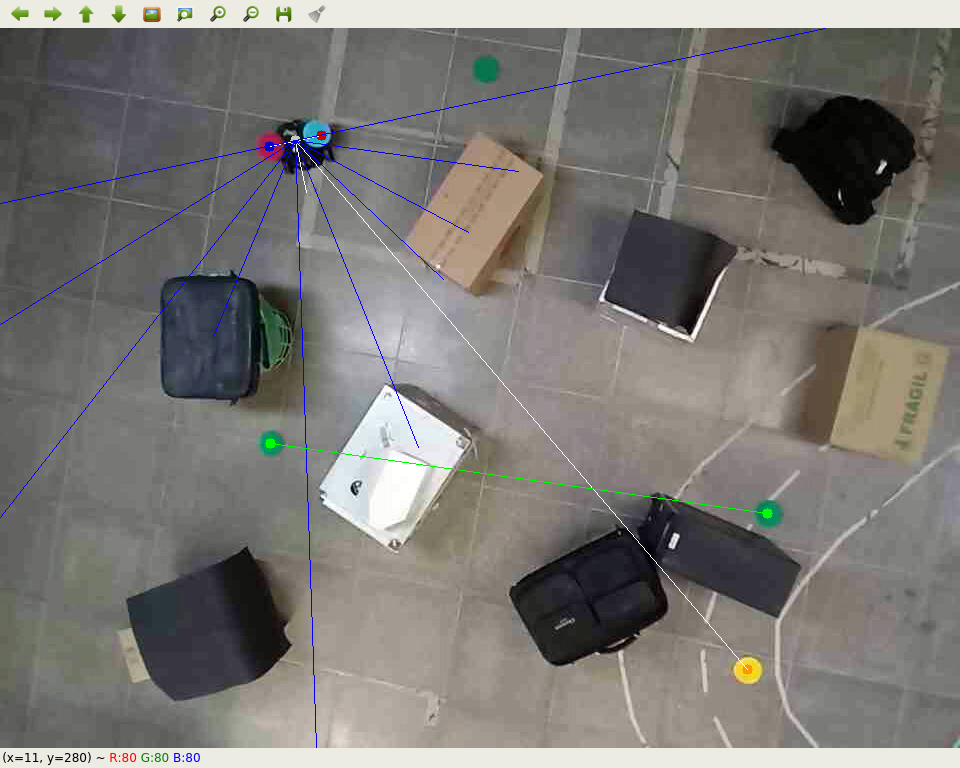
\includegraphics[width=\textwidth]{images/test_env2/1.png}
        \caption{Second real environment.}
        \label{subfig:real_env2}
    \end{subfigure}
    \caption{Environments created for the SAC test on the real world.}\label{fig:real_environments}
\end{figure}